% A LaTeX template for ARTICLE version of the MSc Thesis submissions to 
% Politecnico di Milano (PoliMi) - School of Industrial and Information Engineering
%
% S. Bonetti, A. Gruttadauria, G. Mescolini, A. Zingaro
% e-mail: template-tesi-ingind@polimi.it
%
% Last Revision: October 2021
%
% Copyright 2021 Politecnico di Milano, Italy. Inc. NC-BY

\documentclass[11pt,a4paper]{article} 

%------------------------------------------------------------------------------
%	REQUIRED PACKAGES AND  CONFIGURATIONS
%------------------------------------------------------------------------------
% PACKAGES FOR TITLES
\usepackage{titlesec}
\usepackage{color}

% PACKAGES FOR LANGUAGE AND FONT
\usepackage[utf8]{inputenc}
\usepackage[english]{babel}
\usepackage[T1]{fontenc} % Font encoding

% PACKAGES FOR IMAGES
\usepackage{graphicx}
\graphicspath{{images/}}
\usepackage{eso-pic} % For the background picture on the title page
\usepackage{subfig} % Numbered and caption subfigures using \subfloat
\usepackage{caption} % Coloured captions
\usepackage{transparent}

% STANDARD MATH PACKAGES
\usepackage{amsmath}
\usepackage{amsthm}
\usepackage{bm}
\usepackage[overload]{empheq}  % For braced-style systems of equations

% PACKAGES FOR TABLES
\usepackage{tabularx}
\usepackage{longtable} % tables that can span several pages
\usepackage{colortbl}

% PACKAGES FOR ALGORITHMS (PSEUDO-CODE)
\usepackage{algorithm}
\usepackage{algorithmic}

% PACKAGES FOR REFERENCES & BIBLIOGRAPHY
\usepackage[colorlinks=true,linkcolor=black,anchorcolor=black,citecolor=black,filecolor=black,menucolor=black,runcolor=black,urlcolor=black]{hyperref} % Adds clickable links at references
\usepackage{cleveref}
\usepackage[square, numbers, sort&compress]{natbib} % Square brackets, citing references with numbers, citations sorted by appearance in the text and compressed
\bibliographystyle{plain} % You may use a different style adapted to your field

% PACKAGES FOR THE APPENDIX
\usepackage{appendix}

% PACKAGES FOR ITEMIZE & ENUMERATES 
\usepackage{enumitem}

% OTHER PACKAGES
\usepackage{amsthm,thmtools,xcolor} % Coloured "Theorem"
\usepackage{comment} % Comment part of code
\usepackage{fancyhdr} % Fancy headers and footers
\usepackage{lipsum} % Insert dummy text
\usepackage{tcolorbox} % Create coloured boxes (e.g. the one for the key-words)

%-------------------------------------------------------------------------
%	NEW COMMANDS DEFINED
%-------------------------------------------------------------------------
% EXAMPLES OF NEW COMMANDS -> here you see how to define new commands
\newcommand{\bea}{\begin{eqnarray}} % Shortcut for equation arrays
\newcommand{\eea}{\end{eqnarray}}
\newcommand{\e}[1]{\times 10^{#1}}  % Powers of 10 notation
\newcommand{\mathbbm}[1]{\text{\usefont{U}{bbm}{m}{n}#1}} % From mathbbm.sty
\newcommand{\pdev}[2]{\frac{\partial#1}{\partial#2}}
% NB: you can also override some existing commands with the keyword \renewcommand

%----------------------------------------------------------------------------
%	ADD YOUR PACKAGES (be careful of package interaction)
%----------------------------------------------------------------------------


%----------------------------------------------------------------------------
%	ADD YOUR DEFINITIONS AND COMMANDS (be careful of existing commands)
%----------------------------------------------------------------------------


% Do not change Configuration_files/config.tex file unless you really know what you are doing. 
% This file ends the configuration procedures (e.g. customizing commands, definition of new commands)
% Configuration package
\usepackage[bottom=2.0cm,top=2.0cm,left=2.0cm,right=2.0cm]{geometry}
\raggedbottom 

% Create color bluePoli (-> manuale grafica coordinata:  https://www.polimi.it/fileadmin/user_upload/il_Politecnico/grafica-coordinata/2015_05_11_46xy_manuale_grafica_coordinata.pdf)
\definecolor{bluePoli}{cmyk}{0.4,0.1,0,0.4}

% Custom theorem environments
\declaretheoremstyle[
  headfont=\color{bluePoli}\normalfont\bfseries,
  bodyfont=\color{black}\normalfont\itshape,
]{colored}

\captionsetup[figure]{labelfont={color=bluePoli}} % Set colour of the captions
\captionsetup[table]{labelfont={color=bluePoli}} % Set colour of the captions
\captionsetup[algorithm]{labelfont={color=bluePoli}} % Set colour of the captions

\theoremstyle{colored}
\newtheorem{theorem}{Theorem}[section]
\newtheorem{proposition}{Proposition}[section]

% Enhances the features of the standard "table" and "tabular" environments.
\newcommand\T{\rule{0pt}{2.6ex}}
\newcommand\B{\rule[-1.2ex]{0pt}{0pt}}

% Algorithm description
\newcounter{algsubstate}
\renewcommand{\thealgsubstate}{\alph{algsubstate}}
\newenvironment{algsubstates}{
    \setcounter{algsubstate}{0}%
    \renewcommand{\STATE}{%
    \stepcounter{algsubstate}%
    \Statex {\small\thealgsubstate:}\space}
    }{}
    
% Custom theorem environment
\newcolumntype{L}[1]{>{\raggedright\let\newline\\\arraybackslash\hspace{0pt}}m{#1}}
\newcolumntype{C}[1]{>{\centering\let\newline\\\arraybackslash\hspace{0pt}}m{#1}}
\newcolumntype{R}[1]{>{\raggedleft\let\newline\\\arraybackslash\hspace{0pt}}m{#1}}

% Custom itemize environment
\setlist[itemize,1]{label=$\bullet$}
\setlist[itemize,2]{label=$\circ$}
\setlist[itemize,3]{label=$-$}
\setlist{nosep}

% Create command for background pic
\newcommand\BackgroundPic{% Adding background picture
	\put(237,365){
	    \parbox[b][\paperheight]{\paperwidth}{%
	    \vfill
		\centering
		\transparent{0.4}
		
\includegraphics[width=0.44\paperwidth]{raggiera_polimi.eps}%
		\vfill}
		}
}

% Set indentation
\setlength\parindent{0pt}

% Custom title commands
\titleformat{\section}
{\color{bluePoli}\normalfont\Large\bfseries}
{\color{bluePoli}\thesection.}{1em}{}
\titlespacing*{\section}
{0pt}{3.3ex}{3.3ex}

\titleformat{\subsection}
{\color{bluePoli}\normalfont\large\bfseries}
{\color{bluePoli}\thesubsection.}{1em}{}
\titlespacing*{\subsection}
{0pt}{3.3ex}{3.3ex}

% Custom headers and footers
\pagestyle{fancy}
\fancyhf{}
      
\fancyfoot{}
\fancyfoot[C]{\thepage} % page
\renewcommand{\headrulewidth}{0mm} % headrule width
\renewcommand{\footrulewidth}{0mm} % footrule width

\makeatletter
\patchcmd{\headrule}{\hrule}{\color{black}\hrule}{}{} % headrule
\patchcmd{\footrule}{\hrule}{\color{black}\hrule}{}{} % footrule
\makeatother

% Insert here the info that will be displayed into your Title page 
% -> title of your work
\renewcommand{\title}{TERO PUF Implementation on Xilinx Artix7 FPGA}
% -> abstract (only in English)
\renewcommand{\abstract}{
    Physical Unclonable Functions (PUFs) are becoming important in recent years 
    for various purposes such as Device Identification, True Random Number Generators,
    Cryptographic Key Generators, IP Protection.
    Different ways of realizing PUFs have been proposed in literature, exploiting
    process variations occurring inside chips. 
    Among them, some can be efficiently implemented in FPGAs: in our project, after
    analyzing the state of the art, we chose to implement a Transient Effect Ring Oscillator (TERO) PUF.
    TERO PUF offers high resistance to surrounding logic influence and temperature changes,
    providing at the same time high uniqueness and reliability.
    As target, we chose Basys3 boards from Digilent, shipped with Xilinx Artix7 XC7-A35T.
}

%-------------------------------------------------------------------------
%	BEGIN OF YOUR DOCUMENT
%-------------------------------------------------------------------------
\begin{document}

%-----------------------------------------------------------------------------
% TITLE PAGE
%-----------------------------------------------------------------------------

\AddToShipoutPicture*{\BackgroundPic}

\hspace{-0.6cm}
\includegraphics[width=0.6\textwidth]{logo_polimi_ing_indinf.eps}

\vspace{-1mm}
\Large{\textbf{\color{bluePoli}{\title}}}\\

\vspace{-0.2cm}
\fontsize{0.3cm}{0.5cm}\selectfont \bfseries \textsc{\color{bluePoli} Project Report for Embedded Systems Course}\\

\vspace{-0.2cm}
\large{\textbf{Aspesi Andrea, 962608}} \\
\large{\textbf{Putortì Alessandro, 953258}}

\small \normalfont

\vspace{11pt}

\centerline{\rule{1.0\textwidth}{0.4pt}}

\begin{center}
\begin{minipage}[t]{.24\textwidth}
\begin{minipage}{.90\textwidth}
\noindent
\scriptsize{\textbf{Professors:}} \\
Prof. Fornaciari William \\
Prof. Zoni Davide \\
Prof. Galimberti Andrea \\
\\
\textbf{Academic year:} \\
2021-2022 \\
\\
\end{minipage}
\end{minipage}
\begin{minipage}{.74\textwidth}
\noindent \textbf{\color{bluePoli} Abstract:} {\abstract}
\end{minipage}
\end{center}


%%%%%%%%%%%%%%%%%%%%%%%%%%%%%%
%%    PROJECT MAIN TEXT     %%
%%%%%%%%%%%%%%%%%%%%%%%%%%%%%%

%---------------------------------
% INTRODUCTION
%---------------------------------
%
% Versione Vivado, board e chip 
% che avete preso come target, frequenza operativa, 
% eventuali software aggiuntivi usati.
% Articolo di riferimento implementazione
%
\section{Introduction}
\label{sec:introduction}
Lorem ipsum \textbf{dolor} sit amet, consectetur adipiscing elit. Suspendisse facilisis ac erat vitae luctus. Aliquam in faucibus urna. Nulla ullamcorper tristique odio eu euismod. Nunc porta euismod orci vel ornare. Suspendisse suscipit non orci non blandit. In est massa, blandit sed metus non, commodo euismod leo. Nunc nec purus sed est imperdiet lacinia. Nullam convallis lectus neque, nec gravida \textbf{dolor} semper vel.

Donec quam odio, pulvinar sit amet ipsum et, volutpat ullamcorper ex. Quisque porta, justo nec tempor ornare, leo mauris iaculis ex, sit amet pellentesque quam mi eget neque. Phasellus maximus bibendum sem non pharetra. Morbi elementum tempor sem in scelerisque. Curabitur egestas pharetra libero eget bibendum. Aenean sit amet molestie risus. Quisque ac sodales elit. Nulla tincidunt ac augue vitae malesuada. Proin eget sagittis arcu, non molestie nibh. Nullam in nulla sit amet lacus semper molestie eget eget turpis. Nunc vel urna sit amet nisl facilisis pulvinar in fermentum ligula. Morbi sollicitudin laoreet est eget pharetra. Quisque laoreet porta sem, quis fermentum leo mollis at.

In facilisis viverra felis, a dapibus mauris maximus sed. Curabitur ut eros a odio mollis fermentum vel vel eros. Donec id vestibulum erat, sit amet laoreet urna. Suspendisse aliquam, sapien quis suscipit dapibus, ligula nisl lacinia sem, in tempus neque quam et turpis. Nulla facilisi. Donec malesuada odio sit amet est egestas, in sollicitudin lorem vehicula. Quisque nec dictum quam, vitae tincidunt est. Curabitur id elit fringilla, tincidunt augue ac, pellentesque \textbf{dolor}. Vivamus leo sapien, eleifend eget diam a, porttitor ullamcorper arcu. Donec dignissim ipsum vel sapien porttitor, tincidunt placerat \textbf{dolor} condimentum. Aenean non elementum orci, id molestie nunc. Donec pharetra arcu sem, mollis maximus massa pretium ut. Duis sed congue libero, eu laoreet tortor. Phasellus sed consectetur nisl. Nulla interdum ligula eu placerat porttitor.

%---------------------------------
% DESIGN
%---------------------------------
%
% Breve riassunto del nostro design finale,
% differenze con il loro design, correzioni.
% Funzionamento con challenge, e protocollo comunicazione.
% Challenge disattivate motivo
%
\section{Design}
\label{sec:design}
\subsection{Architecture}
\begin{figure}
    \centering
    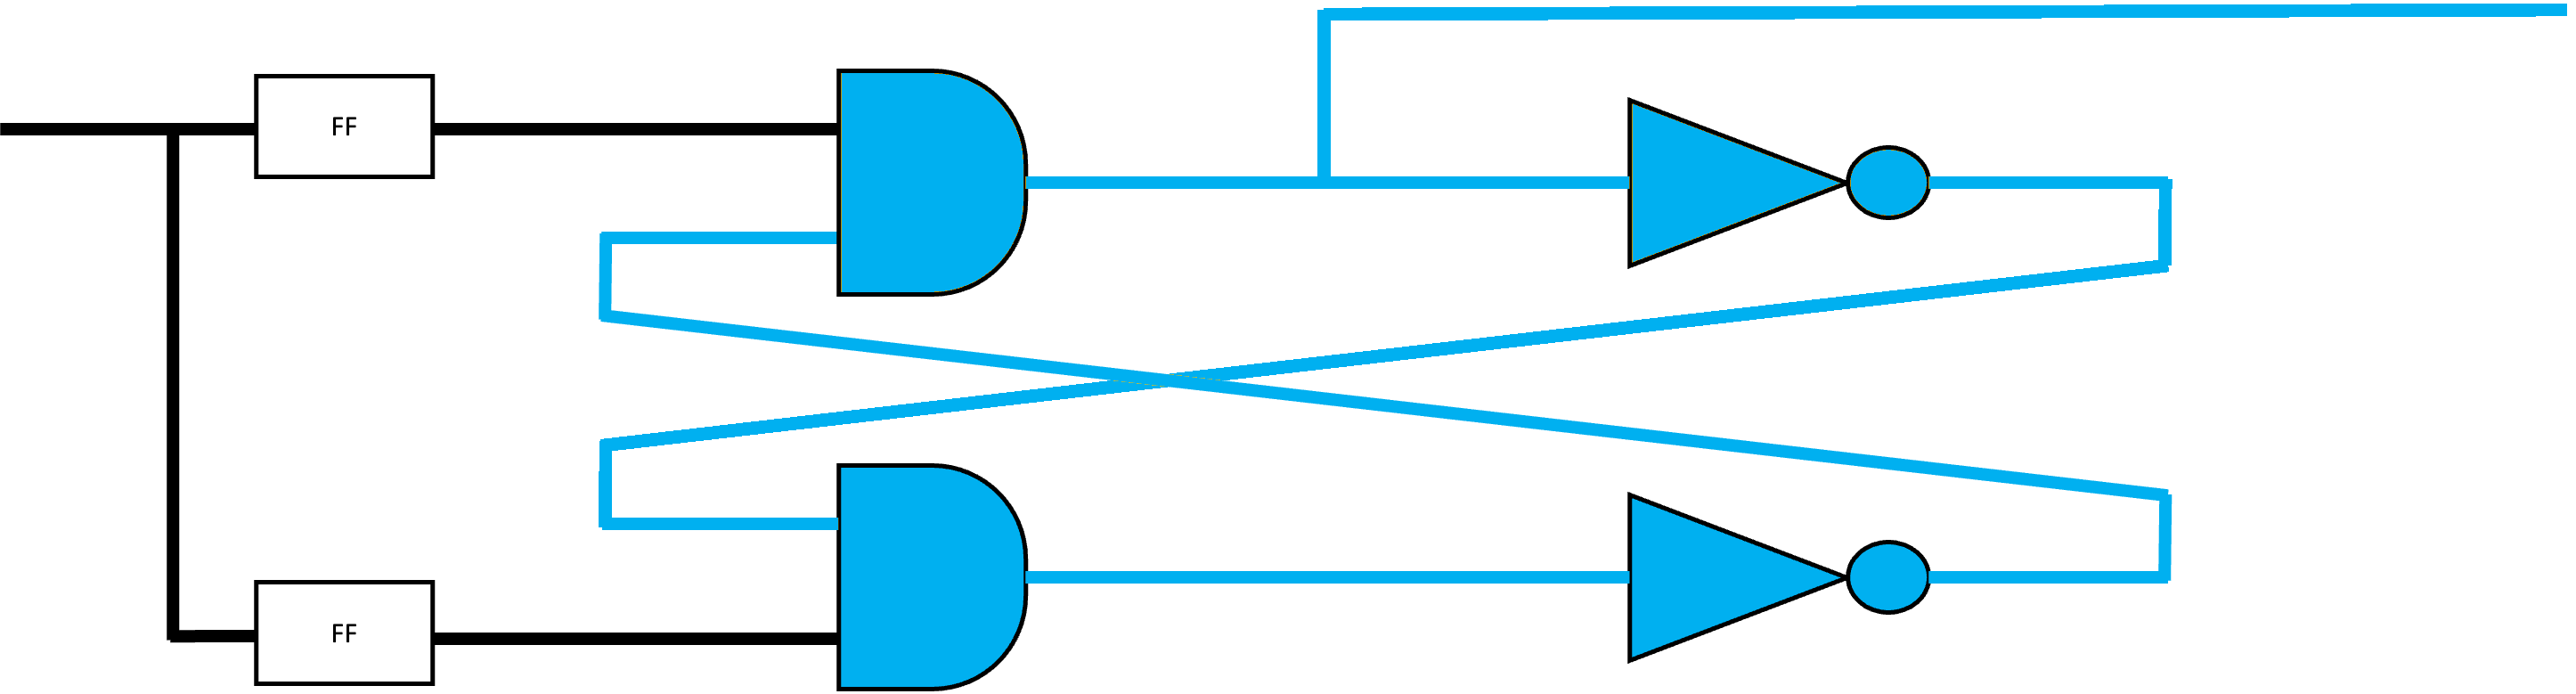
\includegraphics[scale=0.75]{TERO_loop.png}
    \caption{TERO Loop structure}
    \label{img:TERO_LOOP}
\end{figure}
The TERO PUF is composed of a variable number of TERO loops. Each of them is based on
two AND gates and two inverters (see \textit{Figure~\ref{img:TERO_LOOP}}). \\
The two inverters are cross-coupled and brought into an unstable state via AND gates. 
While the loop tries to resolve the unstable state, it oscillates for a short time.
The number of oscillation of each loop is counted using a two-stage counter.
Combining the outcomes of the loops with a specific algorithm (see \textit{Section~\ref{sec:id_generation}}),
we can obtain the overall response of the TERO PUF (ID of the FPGA). \\
In an Artix7 Slice we can put two TERO loops (see \textit{Figure~\ref{img:TERO_CONNECTIONS}}), differing for the internal routing.
These slices are arranged in four adjacent columns, placed in two different positions in the FPGA (see \textit{Figure~\ref{img:TERO_PLACEMENT}}).
\begin{figure}[h]
    \centering
    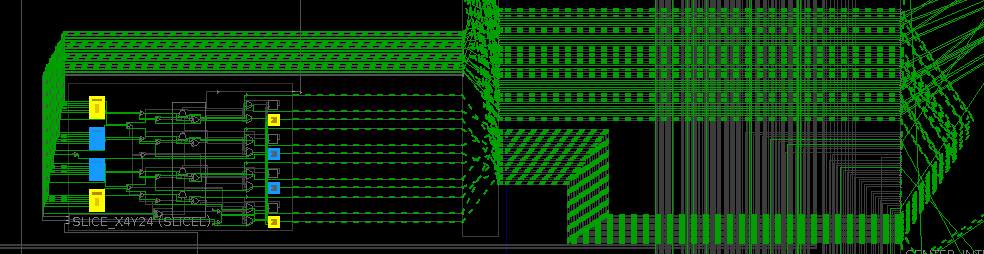
\includegraphics[scale=0.5]{TERO_connections.png}
    \caption{Connection of the two TERO loops inside one Slice}
    \label{img:TERO_CONNECTIONS}
\end{figure} \\
In this way, we obtain eight different types of loops 
(two for the differences at slice-instance times four due to the column arrangement).
Each TERO loop has an enable signal that starts the oscillation when asserted. 
These signals are controlled by an FSM during an evaluation cycle, where each loop is activated and its oscillation measured and averaged.
The evaluation time and the number of measurement used for the average are design parameters (see \textit{Subsection~\ref{subsec:eval_and_repetitions}}).

\subsection{Communication}
The communication with a PC is handled by another FSM, which controls the UART module, 
the FIFO storing the loop responses and the challenge memory. \\
The protocol is the following:
\begin{enumerate}
    \item The PC sends a single byte request to start the interaction.
    \item The PUF replies with a single byte known identifier and waits for a challenge byte.
    \item The PC sends a challenge number encoded in a single byte.
    \item The PUF starts the evaluation of the TERO loops, as specified in details in \textit{Section~\ref{sec:results}}. 
          Each intermediate result is stored in a FIFO queue.
    \item When the evaluation is completed, the FIFO data is sent to the PC all-in-once.
    \item The communication can start again from 1.
\end{enumerate}
To handle the UART communication we exploited open-source Verilog designs found in the
net\footnote{can be found at \href{https://github.com/ben-marshall/uart}{\color{bluePoli}https://github.com/ben-marshall/uart}}, after verifying them.

\subsection{Challenges}
The challenge number sent to the PUF \textbf{could} be used to avoid the evaluation of all the loops.
The needed frequencies are specific to the algorithm used to generate the final response 
(identifier of the FPGA) during the post-processing on the PC. 
At the moment, we decided to expose all the frequencies in order to be able to experiment 
with various algorithms. 

\begin{figure}[H]
    \centering
    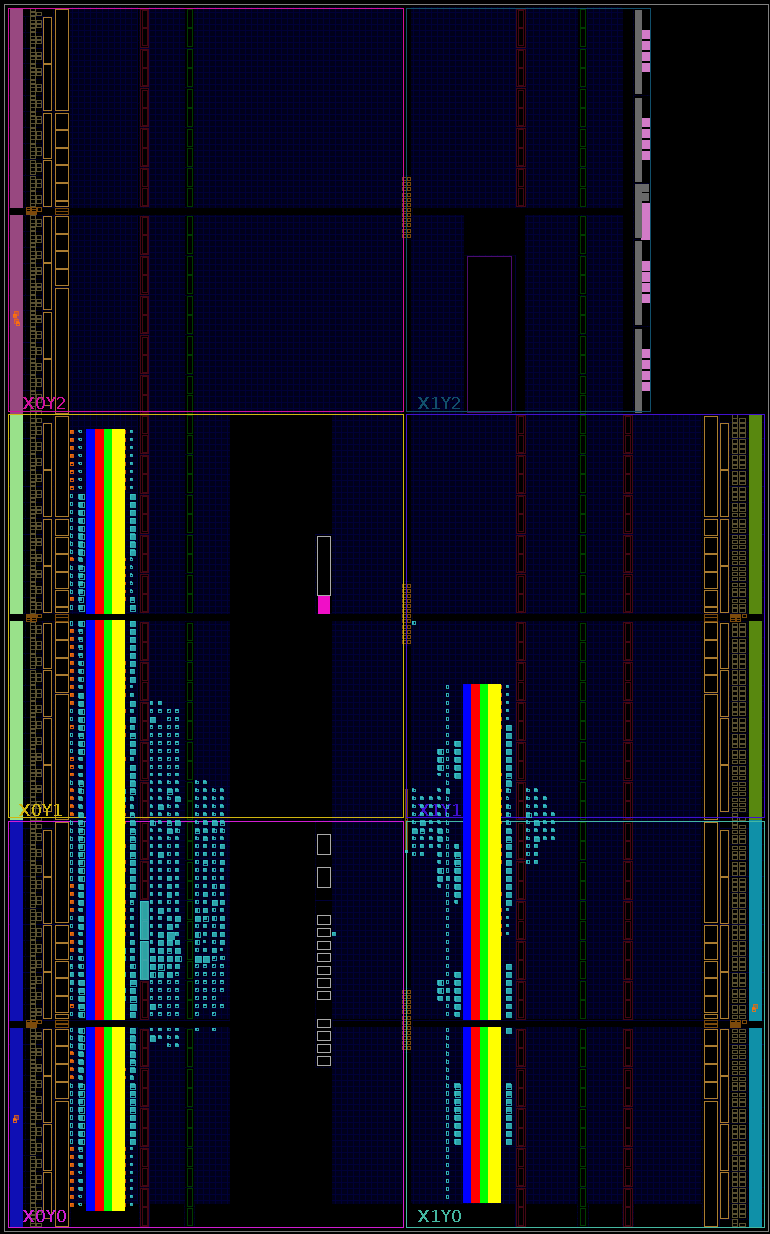
\includegraphics[scale=0.5]{TERO_placement.png}
    \caption{The TERO loops in different columns have different position in relation to the switch matrix, leading to different loop characteristics.}
    \label{img:TERO_PLACEMENT}
\end{figure}

% Sottosezioni
% 1. Architettura: come è composto un tero loop (e come si fa partire), macchine a stati 
% 2. Comunicazione: protocollo interazione via UART
% 3. Challenges: discorso su challenge

%---------------------------------
% IDENTIFICATION ID GENERATION
%---------------------------------
%
% Breve descrizione analisi loro script, differenti
% modalità di generazione ID. Versione scelta da noi (2Comp)
% Pseudo codice generazione con 2Comp
%
\section{ID Generation}
\label{sec:id_generation}
%
% Breve descrizione analisi loro script, differenti
% modalità di generazione ID. Versione scelta da noi (2Comp)
% Pseudo codice generazione con 2Comp
%

As stated in \textit{Section~\ref{sec:design}}, the generation of the ID from the PUF responses can be made in different ways. This choice, naturally,
influences the way the frequencies must be exposed in output (which responses to expose and in which order, given the input challenge). In order to
compare different algorithms we decided to expose in output all the 1280 frequencies, regardless of the challenge. Before computing the actual IDs, we
split the responses in 80 batches of 16 frequencies each. Each batch contains frequencies coming from PUFs of the same type.
In the following some further details about the main algorithms:

\subsection{2Compare}
\label{subsec:2Comp}

2Compare algorithms takes two frequencies, $f_i$ and $f_j$ from each batch, and returns 1 if $f_i > f_j$, else $0$.
Thus, the resulting ID has 80 bits, one for each batch.\\

Below the pseudo-algorithm:

\begin{algorithm}[H]
    \label{alg:2comp}
    \caption{2Compare Algorithm}
    \label{alg:var1}
    \label{protocol11}
    \begin{algorithmic}[1]
    \REQUIRE{$i,j \in [1,16]$, $frequencies(batchIndex,freq)$}
    %\ENSURE { $batchIndex \in [1,80], freq \in [1,16]$}
    %\STATE{$\textbf{Output: } ID [1:80]$}
    \FOR{$batchIndex = 1\ to\ 80$}
    \STATE{$ID[batchIndex] = frequencies(batchIndex,i)>frequencies(batchIndex,j)$}
    \ENDFOR
    \STATE{$return\ \textbf{ID}$}
    \end{algorithmic}
    \end{algorithm} 

After our analysis we stuck to this algorithm since it's easy to implement and the resulting uniqueness and reliability are
are quite good.

\subsection{2Comp Neighbor}
\label{subsec:2Compneigh}

2Compare neighbor is a variation of the previous one. Instead of taking two frequencies for each batch, it compares the
"neighbor" frequencies of the same batch. We decided not to use this algorithm since, with 16 frequencies batches, the
number of bits for each ID is 8, way too low to identify a sufficient number of devices. Increasing the number of frequencies
per batch partially solves this problem, since (for the same number of TERO instances) the number of batches (and thus of challenges)
is consequently reduced.



\subsection{Lehmer-Gray}
\label{subsec:lehmer}

The response generation through Lehmer-Gray encoding is the best in terms of extracted entropy.
allowing to extract 49 bits from a 16 bits batch. It was previously used in \cite{PUFKY}, basing on the method proposed
by Yin and Qu in \cite{YinQu} to extract maximum entropy.

The algorithm consists in computing the Lehmer coefficients $s_i$ for each frequency of a batch, with the following formula:\\

\begin{equation}
    \label{eq:lehmer_coeff}
    % \begin{align}[center]
    s_i = |\{j > i : freq(j)<freq(i)\}|
    % \end{align}
\end{equation}

After that, the obtained coefficients are Gray encoded, and some of the bits of the encoded coefficient are taken as a response.

We did not choose this algorithm since the choice of the bits to take is not trivial, and depends on the particular implementation.



%---------------------------------
% RESULTS E CONCLUSIONS
%---------------------------------
%
% Discutere di valori uniqueness e reliability
% in linea con quelli del paper, discorso su scelta
% evaluation time e repetition bits ed esperimenti.
% Verificati valori del paper originale.
%
\section{Results and Conclusion}
\label{sec:results}
After having realized the design, we transferred it to our two Basys3. \\
With the help of a utility script, we collected frequencies in various configurations. 
In particular, we wanted to verify the best number of repetitions and evaluation time,
in order to have a high reliability, but waiting a reasonable amount of
time for the PUF response. \\
\begin{itemize}
    \item TERO loop are expected to oscillate for a short period of time, then settle in a stable state.
    Using a too short evaluation time truncates the oscillation measurement: although the resulting read
    frequency values display a unique pattern, we can better capture the uniqueness  
    if we wait for most of the loops to stop oscillating. At the same time, a high evaluation time
    can significantly slow down the process, and make the PUF unusable.
    \item Repeating the measurement several times (and averaging the values) is necessary as the
    oscillation frequency of a TERO loop depends, apart from the instance-dependent process variations, on environmental
    noise (e.g., due to temperature or supply voltage differences) and random temporal noise 
    (e.g., temporal fluctuations in the power supply). The latter type is not constant and can be
    averaged out. This approach has been used several times, as it has been proved to increase the reliability
    (as we verified via experiments).
\end{itemize}

\subsection{Evaluation time and Repetitions}

Using the data we collected, we got to the same conclusions of the paper: using more than $ 2^5 $
clock cycles for evaluation does not produce a distinguishable improvement in reliability nor uniqueness 
(as this latter is little influenced by evaluation time). Instead, increasing the number of repetition
from $ 1 $ to $ 2^{12} $ adds an extra $ 5\% $ to the reliability indicator (but slows the response time of the PUF). \\
Using an evaluation time of $ 2^5 $ clock cycles and $ 2^{12} $ repetitions
is the best compromise between reliability and response time of the PUF. \\

\subsection{Reliability}

To calculate the reliability of our implementation, we used 100 measurements each at a different configuration,
comparing the same challenge number response:
\begin{equation}
    Reliability_i = 100\% * (1 - \frac{1}{s} \sum_{t=1}^{s} \frac{HD(Xr_i, X_{i,t})}{n})
\end{equation}
were $ i $ is the i-th challenge (among the 120 available), $ HD $ is the Hamming Distance, $ Xr_i $ is the first response measured 
for that challenge, $ X_{i,t} $ represents each of the 100 responses generated for the i-th challenge, $s=100$ are the measurements taken
and $n=80$ is the number of bits of each response. \\

Using the chosen configuration (evaluation=$ 2^5 $, repetitions=$ 2^{12} $), we got a mean reliability 
of $ 97.4\% $ for the first PUF ($TERO\_AA$), $ 96.9\% $ for the second PUF ($TERO\_AP$). \\
The ideal value for the reliability is $100\%$ (otherwise stated: for each evaluation of the same PUF, fixed the challenge, we would like the same exact response bitwise)

\subsection{Uniqueness}
With the same 100 measurements for the two PUFs of before, we tried to estimate the uniqueness of the response for each given challenge.
Of course to get to a more accurate result, lots of PUFs are required. \\
The formula used for the uniqueness is the following:
\begin{equation}
    Uniqueness_i = 100\% * \frac{k}{k(k-1)} \sum_{i=1}^{k-1}\sum_{j=i+1}^{k} \frac{HD(X_i,X_j)}{n}
\end{equation}
were $ i $ is the i-th challenge (among the 120 available), $k=2$ is the number of PUFs used, $ HD $ is the Hamming Distance, $ X_i $ is the response of the challenge 
for the i-th PUF, $ X_j $ is the response of the challenge for the j-th PUF and $n=80$ is the number of bit of each response. \\

Using the chosen configuration (evaluation=$ 2^5 $, repetitions=$ 2^{12} $), we got a mean uniqueness of $50.25\%$.
The ideal value is $50\%$ (otherwise stated: the probability of a bit flip between two responses of different PUFs, fixed the challenge, is $50\%$ - the toss of a coin).

\subsection{Conclusion}
Seen such results, we consider the implementation of the TERO PUF successful, and in line with the results of the paper. \\
Further work can be done to use the challenge directly in the FPGA to send only the needed frequency measurements, and in this way avoid
exposing the whole CRP (i.e. Challenge Response) space. As anticipated in the design, little effort is required to achieve this with our implementation.

\newpage
\
\newpage
\
\newpage

%-----------------------------------------------------------------------------
% INTRODUCTION
%-----------------------------------------------------------------------------
\section{Introduction}
\label{sec:introduction}
This document is intended to be both an example of the Polimi \LaTeX{} template for Master Theses in article format,
as well as a short introduction to its use. It is not intended to be a general introduction to \LaTeX{} itself,
and the reader is assumed to be familiar with the basics of creating and compiling \LaTeX{} documents (see \cite{oetiker1995not, kottwitz2015latex}). 
\\
The cover page of the thesis in article format must contain all the relevant information:
title of the thesis, name of the Study Programme, name(s) of the author(s),
student ID number, name of the supervisor, name(s) of the co-supervisor(s) (if any), academic year.
\\
Be sure to select a title that is meaningful.
It should contain important keywords to be identified by indexer.
Keep the title as concise as possible and comprehensible even to people who are not experts in your field.
The title has to be chosen at the end of your work so that it accurately captures the main subject of the manuscript.

It is convenient to break the article format of your thesis (in article format) into sections and subsections. 
If necessary, subsubsections, paragraphs and subparagraphs can be used. 
A new section is created by the command
\begin{verbatim}
\section{Title of the section}
\end{verbatim}
The numbering can be turned off by using \verb|\section*{}|.
A new subsection is created by the command
\begin{verbatim}
\subsection{Title of the subsection}
\end{verbatim}
and, similarly, the numbering can be turned off by adding an asterisk as follows 
\begin{verbatim}
\subsection*{}
\end{verbatim}
It is recommended to give a label to each section by using the command
\begin{verbatim}
\label{sec:section_name}%
\end{verbatim}
where the argument is just a text string that you'll use to reference that part
as follows: \textit{Section~\ref{sec:introduction} contains \sc{INTRODUCTION}  \dots}.

%-----------------------------------------------------------------------------
% EQUATIONS
%-----------------------------------------------------------------------------
\section{Equations}
\label{sec:eqs}
This section gives some examples of writing mathematical equations in your thesis.

Maxwell's equations read:
\begin{subequations}
    \label{eq:maxwell}
    \begin{align}[left=\empheqlbrace]
    \nabla\cdot \bm{D} & = \rho, \label{eq:maxwell1} \\
    \nabla \times \bm{E} +  \frac{\partial \bm{B}}{\partial t} & = \bm{0}, \label{eq:maxwell2} \\
    \nabla\cdot \bm{B} & = 0, \label{eq:maxwell3} \\
    \nabla \times \bm{H} - \frac{\partial \bm{D}}{\partial t} &= \bm{J}. \label{eq:maxwell4}
    \end{align}
\end{subequations}

Equation~\eqref{eq:maxwell} is automatically labeled by \texttt{cleveref},
as well as Equation~\eqref{eq:maxwell1} and Equation~\eqref{eq:maxwell3}.
Thanks to the \verb|cleveref| package, there is no need to use \verb|\eqref|.
Equations have to be numbered only if they are referenced in the text.

Equations~\eqref{eq:maxwell_multilabels1}, \eqref{eq:maxwell_multilabels2}, \eqref{eq:maxwell_multilabels3}, and \eqref{eq:maxwell_multilabels4} show again Maxwell's equations without brace:
\begin{align}
    \nabla\cdot \bm{D} & = \rho, \label{eq:maxwell_multilabels1} \\
    \nabla \times \bm{E} +  \frac{\partial \bm{B}}{\partial t} &= \bm{0}, \label{eq:maxwell_multilabels2} \\
    \nabla\cdot \bm{B} & = 0, \label{eq:maxwell_multilabels3} \\
    \nabla \times \bm{H} - \frac{\partial \bm{D}}{\partial t} &= \bm{J} \label{eq:maxwell_multilabels4}.
\end{align}

Equation~\eqref{eq:maxwell_singlelabel} is the same as before,
but with just one label:
\begin{equation}
    \label{eq:maxwell_singlelabel}
    \left\{
    \begin{aligned}
    \nabla\cdot \bm{D} & = \rho, \\
    \nabla \times \bm{E} +  \frac{\partial \bm{B}}{\partial t} &= \bm{0},\\
    \nabla\cdot \bm{B} & = 0, \\
    \nabla \times \bm{H} - \frac{\partial \bm{D}}{\partial t} &= \bm{J}.
    \end{aligned}
    \right.
\end{equation}

%-----------------------------------------------------------------------------
% FIGURES, TABLES AND ALGORITHMS
%-----------------------------------------------------------------------------
\section{Figures, Tables and Algorithms}

Figures, Tables and Algorithms have to contain a Caption that describes their content, and have to be properly referred in the text.

\subsection{Figures}
\label{subsec:figures}

For including pictures in your text you can use \texttt{TikZ} for high-quality hand-made figures \cite{tikz},
or just include them with the command
\begin{verbatim}
\includegraphics[options]{filename.xxx}
\end{verbatim}
Here xxx is the correct format, e.g.  \verb|.png|, \verb|.jpg|, \verb|.eps|, \dots.

\begin{figure}[H]
    \centering
    
\includegraphics[width=0.3\textwidth]{logo_polimi_scritta.eps}
    \caption{Caption of the Figure.}
    \label{fig:quadtree}
\end{figure}

Thanks to the \texttt{\textbackslash subfloat} command, a single figure, such as Figure~\ref{fig:quadtree},
can contain multiple sub-figures with their own caption and label, e.g. Figure~\ref{fig:polimi_logo1} and Figure~\ref{fig:polimi_logo2}. 

\begin{figure}[H]
    \centering
    \subfloat[One PoliMi logo.\label{fig:polimi_logo1}]{
        
\includegraphics[scale=0.5]{images/logo_polimi_scritta.eps}
    }
    \quad
    \subfloat[Another one PoliMi logo.\label{fig:polimi_logo2}]{
        
\includegraphics[scale=0.5]{images/logo_polimi_scritta2.eps}
    }
    \caption[]{Caption of the Figure.}
    \label{fig:quadtree2}
\end{figure}

\subsection{Tables}
\label{subsec:tables}

Within the environments \texttt{table} and  \texttt{tabular} you can create very fancy tables as the one shown in Table~\ref{table:example}.

\begin{table}[H]
    \caption*{\textbf{Example of Table (optional)}}
    \centering 
    \begin{tabular}{|p{3em} c c c |}
    \hline
    \rowcolor{bluePoli!40}
     & \textbf{column1} & \textbf{column2} & \textbf{column3} \T\B \\
    \hline \hline
    \textbf{row1} & 1 & 2 & 3 \T\B \\
    \textbf{row2} & $\alpha$ & $\beta$ & $\gamma$ \T\B\\
    \textbf{row3} & alpha & beta & gamma \B\\
    \hline
    \end{tabular}
    \\[10pt]
    \caption{Caption of the Table.}
    \label{table:example}
\end{table}

You can also consider to highlight selected columns or rows in order to make tables more readable.
Moreover, with the use of \texttt{table*} and the option \texttt{bp} it is possible to align them at the bottom of the page. One example is presented in Table~\ref{table:exampleC}. 

\begin{table*}[bp]
\centering 
    \begin{tabular}{|p{3em} | c | c | c | c | c | c|}
    \hline
%    \rowcolor{bluePoli!40}
     & \textbf{column1} & \textbf{column2} & \textbf{column3} & \textbf{column4} & \textbf{column5} & \textbf{column6} \T\B \\
    \hline \hline
    \textbf{row1} & 1 & 2 & 3 & 4 & 5 & 6 \T\B\\
    \textbf{row2} & a & b & c & d & e & f \T\B\\
    \textbf{row3} & $\alpha$ & $\beta$ & $\gamma$ & $\delta$ & $\phi$ & $\omega$ \T\B\\
    \textbf{row4} & alpha & beta & gamma & delta & phi & omega \B\\
    \hline
    \end{tabular}
    \\[10pt]
    \caption{Highlighting the columns}
    \label{table:exampleC}
\end{table*}

\subsection{Algorithms}
\label{subsec:algorithms}

Pseudo-algorithms can be written in \LaTeX{} with the \texttt{algorithm} and \texttt{algorithmic} packages.
An example is shown in Algorithm~\ref{alg:var}.
\begin{algorithm}[H]
\label{alg:example}
\caption{Name of the Algorithm}
\label{alg:var}
\label{protocol1}
\begin{algorithmic}[1]
\STATE Initial instructions
\FOR{$for-condition$}
\STATE{Some instructions}
\IF{$if-condition$}
\STATE{Some other instructions}
\ENDIF
\ENDFOR
\WHILE{$while-condition$}
\STATE{Some further instructions}
\ENDWHILE
\STATE Final instructions
\end{algorithmic}
\end{algorithm} 

\section{Some further useful suggestions}

Theorems have to be formatted as follows:
\begin{theorem}
\label{a_theorem}
Write here your theorem. 
\end{theorem}
\textit{Proof.} If useful you can report here the proof.
\vspace{0.3cm} % Insert vertical space

Propositions have to be formatted as follows:
\begin{proposition}
Write here your proposition.
\end{proposition}
\vspace{0.3cm} % Insert vertical space

How to insert itemized lists:
\begin{itemize}
    \item first item;
    \item second item.
\end{itemize}
How to write numbered lists:
\begin{enumerate}
    \item first item;
    \item second item.
\end{enumerate}

\section{Use of copyrighted material}

Each student is responsible for obtaining copyright permissions, if necessary, to include published material in the thesis.
This applies typically to third-party material published by someone else.

\section{Plagiarism}

You have to be sure to respect the rules on Copyright and avoid an involuntary plagiarism.
It is allowed to take other persons' ideas only if the author and his original work are clearly mentioned.
As stated in the Code of Ethics and Conduct, Politecnico di Milano \textit{promotes the integrity of research,
condemns manipulation and the infringement of intellectual property}, and gives opportunity to all those
who carry out research activities to have an adequate training on ethical conduct and integrity while doing research.
To be sure to respect the copyright rules, read the guides on Copyright legislation and citation styles available
at:
\begin{verbatim}
https://www.biblio.polimi.it/en/tools/courses-and-tutorials
\end{verbatim}
You can also attend the courses which are periodically organized on "Bibliographic citations and bibliography management".

%-----------------------------------------------------------------------------
% CONCLUSION
%-----------------------------------------------------------------------------
\section{Conclusions}
\color{black}
A final section containing the main conclusions of your research/study
and possible future developments of your work have to be inserted in the section ``Conclusions''.

\section{Bibliography and citations}
Your thesis must contain a suitable Bibliography which lists all the sources consulted on developing the work.
The list of references is placed at the end of the manuscript after the chapter containing the conclusions.
It is suggested to use the BibTeX package and save the bibliographic references in the file \verb|bibliography.bib|.
This is indeed a database containing all the information about the references. To cite in your manuscript, use the \verb|\cite{}| command as follows:
\\
\textit{Here is how you cite bibliography entries: \cite{knuth74}, or multiple ones at once: \cite{knuth92,lamport94}}.
\\
The bibliography and list of references are generated automatically by running BibTeX \cite{bibtex}.

%-----------------------------------------------------------------------------
% BIBLIOGRAPHY
%-----------------------------------------------------------------------------
\bibliography{bibliography.bib}

\appendix
\section{Appendix A}
If you need to include an appendix to support the research in your thesis, you can place it at the end of the manuscript.
An appendix contains supplementary material (figures, tables, data, codes, mathematical proofs, surveys, \dots)
which supplement the main results contained in the previous sections.

\section{Appendix B}
It may be necessary to include another appendix to better organize the presentation of supplementary material.

%%%%%%%%%%%%%%%%%%%%%%%%%%%%%%%%%%%%%%%%%%%%%%%%%%%%%%%%%%%%%%
%%     ABSTRACT IN ITALIAN LANGUAGE AND ACKNOWLEDGMENTS     %%
%%%%%%%%%%%%%%%%%%%%%%%%%%%%%%%%%%%%%%%%%%%%%%%%%%%%%%%%%%%%%%
\cleardoublepage

%-----------------------------------------------------------------------------
% SOMMARIO
%-----------------------------------------------------------------------------
\section*{Abstract in lingua italiana}
Qui va l'Abstract in lingua italiana della tesi seguito dalla lista di parole chiave.
\vspace{15pt}
\begin{tcolorbox}[arc=0pt, boxrule=0pt, colback=bluePoli!60, width=\textwidth, colupper=white]
    \textbf{Parole chiave:} qui, le parole chiave, della tesi, in italiano 
\end{tcolorbox}

%-----------------------------------------------------------------------------
% ACKNOWLEDGEMENTS
%-----------------------------------------------------------------------------
\section*{Acknowledgements}
Here you might want to acknowledge someone.

%-------------------------------------------------------------------------
%	END OF YOUR DOCUMENT
%-------------------------------------------------------------------------
\end{document}